% !TEX TS-program = xelatexmk

\documentclass[12pt]{myNotes}

%%%%%%%%%%%%%%%%%%%%%%%%%%%%%%%%%%%%%%%%%%%%%%%%%%%%%%%%%%%%%%%%%%%%%%%%%%%
\usepackage[english]{babel}
\hyphenation{TOPPView}
\hyphenation{KNIME}
\hyphenation{OpenMS}
\hyphenation{X!Tandem}
\hyphenation{XTandem-Adapter}

%%%%%%%%%%%%%%%%%%%%%%%%%%%%%%%%%%%%%%%%%%%%%%%%%%%%%%%%%%%%%%%%%%%%%%%%%%%
% FONT SELECTION -> WE NOW USE UBUNTU FONT AND XETEX FOR A MORE PROFESSIONAL
% LOOK.
% UBUNTU FONT CAN BE DOWNLOADED FROM HERE: http://font.ubuntu.com
%
\usepackage{fontspec}

\setmainfont[Ligatures = TeX]{Ubuntu-R.ttf}

\setmonofont[Ligatures = TeX]{Ubuntu-M.ttf}
% math fonts
%\usepackage[math-style=TeX]{unicode-math}
%\setmathfont{Cambria Math}


%%%%%%%%%%%%%%%%%%%%%%%%%%%%%%%%%%%%%%%%%%%%%%%%%%%%%%%%%%%%%%%%%%%%%%%%%%%
\usepackage{amsmath,amssymb,amscd,bm,dsfont,wasysym}
\usepackage{graphicx}
\usepackage[xetex,
      colorlinks=false,
      urlcolor=black,       % \href{...}{...} external (URL)
      filecolor=black,     % \href{...} local file
      linkcolor=black,       % \ref{...} and \pageref{...}
      citecolor=black,
      pdftitle={GCB Tutorial Handouts},
      pdfauthor={Timo Sachsenberg},
      pdfsubject={},
      pdfkeywords={},
      pagebackref,
      pdfpagemode=none,
      bookmarksopen=true]{hyperref}

%%%%%%%%%%%%%%%%%%%%%%%%%%%%%%%%%%%%%%%%%%%%%%%%%%%%%%%%%%%%%%%%%%%%%%%%%%%

\newfontfamily{\menlo}{Menlo-Regular.ttf}

\usepackage{listings}
\usepackage{color}
\usepackage{textcomp}
\definecolor{listinggray}{gray}{0.9}
\definecolor{lbcolor}{rgb}{0.9,0.9,0.9}
\lstset{
    backgroundcolor=\color{lbcolor},
    tabsize=4,
    rulecolor=,
    language=python,
    basicstyle=\menlo\scriptsize,
    upquote=true,
    aboveskip={1.5\baselineskip},
    columns=fixed,
    showstringspaces=false,
    extendedchars=true,
    breaklines=true,
    prebreak = \raisebox{0ex}[0ex][0ex]{\ensuremath{\hookleftarrow}},
    frame=single,
    showtabs=false,
    showspaces=false,
    showstringspaces=false,
    identifierstyle=\menlo,
    keywordstyle=\color[rgb]{0,0,1},
    commentstyle=\color[rgb]{0.133,0.545,0.133},
    stringstyle=\color[rgb]{0.627,0.126,0.941},
}

%%%%%%%%%%%%%%%%%%%%%%%%%%%%%%%%%%%%%%%%%%%%%%%%%%%%%%%%%%%%%%%%%%%%%%%%%%%
% only use those two in combination
\usepackage[textsize=scriptsize]{todonotes}
%\usepackage[firstpage]{draftwatermark}
%\SetWatermarkScale{4}

%%%%%%%%%%%%%%%%%%%%%%%%%%%%%%%%%%%%%%%%%%%%%%%%%%%%%%%%%%%%%%%%%%%%%%%%%%%
% better key and menu tips
\usepackage{menukeys}
\renewmenumacro{\directory}[/]{pathswithfolder}

%%%%%%%%%%%%%%%%%%%%%%%%%%%%%%%%%%%%%%%%%%%%%%%%%%%%%%%%%%%%%%%%%%%%%%%%%%%
% easy referencing
\usepackage[noabbrev,capitalise]{cleveref}

%%%%%%%%%%%%%%%%%%%%%%%%%%%%%%%%%%%%%%%%%%%%%%%%%%%%%%%%%%%%%%%%%%%%%%%%%%%
% subfigures
\usepackage{subcaption}

%%%%%%%%%%%%%%%%%%%%%%%%%%%%%%%%%%%%%%%%%%%%%%%%%%%%%%%%%%%%%%%%%%%%%%%%%%%
% boxes with notes
%%%%%%%%%%%%%%%%%%%%%%%%%%%%%%%%%%%%%%%%%%%%%%%%%%%%%%%%%%%%%%%%%%%%%%%%%%%
\usepackage{tikz}
\usetikzlibrary[shadows]
\usepackage[framemethod=TikZ]{mdframed}
\usetikzlibrary{calc}

\global\mdfdefinestyle{notedefault}{topline=false,bottomline=false,rightline=false,leftmargin=1cm}
\newcommand{\note}[1]{ \begin{mdframed}[style=notedefault] \textbf{Note:}~#1 \end{mdframed} }

%%%%%%%%%%%%%%%%%%%%%%%%%%%%%%%%%%%%%%%%%%%%%%%%%%%%%%%%%%%%%%%%%%%%%%%%%%%
\newmdenv[
  leftmargin=0pt,
  rightmargin=20pt,
  innertopmargin=30pt,
  innerbottommargin=10pt,
  innerleftmargin=45pt,
  middlelinewidth=0pt,
  linecolor=black,
  topline=false,
  bottomline=false,
  rightline=false,
  font=\normalfont\normalsize,
  frametitlefont=\normalfont\normalsize\bfseries,
  frametitleaboveskip=1em,
  singleextra={
    \node[inner sep=0pt,anchor=north west,xshift=10pt,yshift=-30pt] at (P-|O) {\includegraphics[width=1.3cm]{graphics/assets/question23}};
    \node[inner sep=0pt,anchor=north west,yshift=-.8\baselineskip,font=\bfseries,xshift=10pt] at (P-|O) {Question};
  },
  firstextra={
    \node[inner sep=0pt,anchor=north west,xshift=10pt,yshift=-30pt] at (P-|O) {\includegraphics[width=1.3cm]{graphics/assets/question23}};
    \node[inner sep=0pt,anchor=north west,yshift=-.8\baselineskip,font=\bfseries,xshift=10pt] at (P-|O) {Question};
  }
]{question}

%%%%%%%%%%%%%%%%%%%%%%%%%%%%%%%%%%%%%%%%%%%%%%%%%%%%%%%%%%%%%%%%%%%%%%%%%%%
\newmdenv[
  leftmargin=0pt,
  rightmargin=20pt,
  innertopmargin=30pt,
  innerbottommargin=10pt,
  innerleftmargin=45pt,
  middlelinewidth=0pt,
  linecolor=black,
  topline=false,
  bottomline=false,
  rightline=false,
  font=\normalfont\normalsize,
  frametitlefont=\normalfont\normalsize\bfseries,
  frametitleaboveskip=1em,
  singleextra={
    \node[inner sep=0pt,anchor=north west,xshift=10pt,yshift=-30pt] at (P-|O) {\includegraphics[width=1.3cm]{graphics/assets/check30}};
    \node[inner sep=0pt,anchor=north west,yshift=-.8\baselineskip,font=\bfseries,xshift=10pt] at (P-|O) {Task};
  },
  firstextra={
    \node[inner sep=0pt,anchor=north west,xshift=10pt,yshift=-30pt] at (P-|O) {\includegraphics[width=1.3cm]{graphics/assets/check30}};
    \node[inner sep=0pt,anchor=north west,yshift=-.8\baselineskip,font=\bfseries,xshift=10pt] at (P-|O) {Task};
  }
]{task}

%%%%%%%%%%%%%%%%%%%%%%%%%%%%%%%%%%%%%%%%%%%%%%%%%%%%%%%%%%%%%%%%%%%%%%%%%%%
\newcommand{\KNIMENODE}[1]{\texttt{#1}}
\newcommand{\OPENMSTOOL}[1]{\texttt{#1}}

\begin{document}
%%%%%%%%%%%%%%%%%%%%%%%%%%%%%%%%%%%%%%%%%%%%%%%%%%%%%%%%%%%%%%%%%%%%%%%%%%%

\firstpages

%%%%%%%%%%%%%%%%%%%%%%%%%%%%%%%%%%%%%%%%%%%%%%%%%%%%%%%%%%%%%%%%%%%%%%%%%%%

\setcounter{equation}{0}

%%%%%%%%%%%%%%%%%%%%%%%%%%%%%%%%%%%%%%%%%%%%%%%%%%%%%%%%%%%%%%%%%%%%%%%%%%%
%\newpage

%!TEX root = handout.tex

\section{General remarks}
\label{General remarks}

\begin{itemize}
\item This handout will guide you through the tutorial ``Fundamentals of Proteome Bioinformatics Revisited''.
\item In this hands-on tutorial session, you will become familiar with some of the tutorial topics with hands-on and homework and the basic functionalities of KNIME and OpenMS/TOPP, as well as learn how to use a selection of TOPP tools used in the tutorial workflows.
\item OpenMS~\cite{Sturm2008} is a versatile open-source library for mass spectrometry data analysis. Based on this library, we offer a collection
      of command-line tools ready to be used by end users. These so-called TOPP tools (short for ``The OpenMS Proteomics Pipeline'')~\cite{Kohlbacher2007} can be understood as
      small building blocks of arbitrary complex data analysis workflows.
\item In order to facilitate workflow construction, OpenMS was integrated into KNIME~\cite{KNIME}, the Konstanz
			Information Miner, an open-source integration platform providing a powerful and flexible workflow system
			combined with advanced data analytics, visualisation, and report capabilities. Raw MS data as well as the
			results of data processing using TOPP can be visualized using TOPPView~\cite{Sturm2009}.
\item All data referenced in this tutorial can be found in the \directory{Example\_Data} folder that came with this tutorial.
%\item Installation packages of the new OpenMS 1.11 release for Windows (32 and 64 bit) and Mac OS X (10.7 and 10.8) as well as
%      all data required for this tutorial session can be found on the USB sticks provided by us.
\end{itemize}


\setcounter{equation}{0}

\newpage{}

%!TEX root = handout.tex

\section{Session 1 - Sequence databases}
\label{Session 1 - Sequence databases}
\begin{task}

The following tasks are a good starting point to get used with sequence database handling in Protoemics. Some questions don't have yes / no answers, but need differentiation.
\begin{enumerate}
\item How long are the sequences of human GAPDH (isoform-1) in GenBank and UniProtKB/SwissProt? What is/are the reason(s) for the difference in length?
\item How many sequence isoforms has the human protein "sorcin" in \mbox{UniProtKB}/ SwissProt? In which sequence positions / ranges do they differ? What reason is given for the different isoforms?
\item Are ApoB variants ApoB-48 and ApoB-100 (due to RNA-Editing) stored as sequence isoforms in UniProtKB/SwissProt?
\item Are all SNPs of Glucokinase shown in GenBank (or their amino acid changes in UniProtKB/SwissProt?
\item What is the problem with the regular expression \verb+>sp|\([^|]*\)+ when used for parsing of accessions in uniprot\_complete-mus\_musculus.fasta (here \verb+\(+ and \verb+\)+ are used for accessing the contents of a sub-expression)?
\item How many sequences are contained in the 2015\_9 release of UniProtKB human complete reference  proteome set, both without isoforms and with isoforms?
\item Download the UniprotKB complete reference proteome set of the sea snail Lottia gigantea as FASTA. How many sequences are in the FASTA? How many are from SwissProt and how many from TrEMBL?
\item Why are in the UniProtKB human complete reference proteome set (which contains protein sequences of SwissProt and TrEMBL for all known human genes) less SwissProt sequences than in the human UniProtKB/SwissProt FASTA itself?

\end{enumerate}
\end{task}

\newpage{}

\include{introduction_knime}
\newpage{}

%!TEX root = handout.tex

\section{Session 2 - The target-decoy approach}
In this part of the tutorial session two exercises regarding the manual computation of the target-decoy approach (TDA) will be conducted. Nowadays these tasks are performed automatically and "behind the scenes" by proteomics software tools and workflow engines. However, it is recommended to apply the TDA for some search engine results manually in order to get a better insight into the crucial FDR estimation for PSM identification.
\begin{figure}[ht]
	\centering
		\includegraphics[scale=0.9]{graphics/targetdecoy/decoydatabasebuilder.png}
	\label{fig:decoydatabasebuilder}
	\caption{Screenshot of the tool \texttt{DecoyDatabaseBuilder}}
\end{figure}



\subsection{Exercise 1: Generate decoy databases}
Nowadays, the construction of decoy databases (decoy DBs) as well as the whole TDA and FDR estimation are hidden features of large proteomics software. Nevertheless, specific software tools are recommended and still in use in many labs in order to construct decoy DBs alternatively (in a way not supported by the large software used in the lab) or to perform a custom FDR estimation (e.g. different equations or different strategies for decoy generation). The \texttt{DecoyDatabaseBuilder} provided by the MPC is such a specific software for decoy DB construction. The java tool can be download from \menu{http://www.ruhr-uni-bochum.de/mpc/software/DecoyBuilder/index.html}. For this tutorial, the DecoyDatabaseBuilder can be found on the USB key.

\begin{task}
In order to construct decoy DBs please start the DecoyDatabaseBuilder by clicking on \texttt{DecoyDatabaseBuilder.jar}. Then, process the following DBs that are needed for the TDA-related workflows coming with this tutorial:
\begin{itemize}
	\item \directory{isb18mix.fasta}: by clicking \menu{reverse \& append Fasta...} and choosing this DB file (i.e., FASTA-file) please create a target-decoy DB by concatenation of the original DB and the DB of its reversed sequences.
	\item \directory{isb18mix.fasta} (again): by clicking \menu{shuffle \& append Fasta...} and choosing this DB file (i.e., FASTA-file) please create a target-decoy DB by concatenation of the original DB and the DB of its shuffled sequences.
	\item \directory{isb18\_plus\_yeast\_mod.fasta}: by clicking \menu{reverse \& append Fasta...} and choosing this DB file (i.e., FASTA-file) please create a target-decoy DB by concatenation of the original DB and the DB of its reversed sequences.
\end{itemize}
You will find the original FASTA-files on the flash drive (subfolder \newline{}\directory{databases\_and\_spectra} in the folder for this session). Please check the results that will be automatically saved in the source file folder by opening and inspecting them in a text editor (the basic notepad will not work, you can use e.g. Notepad++ or Vim)!
\end{task}



\subsection{Exercise 2: Load and run a KNIME-workflow for testing FDR formulas}
\textbf{Execute KNIME-workflow:} Switch to the workflow "GCB2015 I-3". Please correct your input and output paths for the nodes \KNIMENODE{Input File} (paths to the FASTA-file and the mzXML-file that can be found in the subfolder \directory{databases\_and\_spectra}) and \KNIMENODE{Output File} (e.g., the output folder \directory{exercise2} on the flash drive). Then, please run the workflow and check the two resulting csv files.

\begin{figure}
	\centering
		\includegraphics[scale=0.7]{graphics/targetdecoy/workflow_tda_i3.png}
	\label{fig:workflow_tda_i3}
	\caption{KNIME-workflow for exercise 2}
\end{figure}

\begin{task}

\texttt{Compute FDRs for X!Tandem results:} Now load the spectrum identification results csv file of the search engine "X!Tandem" (KNIME node: "XTandemAdapter") as well as the TDA template file "tda\_I3.xlsx" in Excel. Sort the data by means of the search engine score (here: from large to small values). In the highlighted columns of the template file the FDR estimation via TDA is performed. So, please apply the respective formulas given in the template to the X!Tandem results file.

\texttt{Compute FDRs for MS-GF+ results:} Now load the spectrum identification results csv file of the search engine "MS-GF+" (KNIME node: "MSGFPlusAdapter") as well as the TDA template file "tda\_I3.xlsx" in Excel. Sort the data by means of the search engine score (here: from small to large values). In the highlighted columns of the template file the FDR estimation via TDA is performed. So, please apply the respective formulas given in the template to the MS-GF+ results file.

\texttt{Explanation of the TDA-related columns in the template file:} In the following the columns of the TDA template file are explained:
\begin{itemize}
	\item \texttt{isDecoy:} For each position in the sorted data the current protein accession is checked whether it contains a specific tag indicating decoys proteins (e.g., in the example files "e" for reverse or "s" for shuffle). These tags are attached to decoy accessions by tools constructing decoy DBs.
	\item \texttt{decoyCount:} For each position of the sorted data the current number of decoys (i.e., $N_{decoys}$).
	\item \texttt{PSMcount:} For each position of the sorted data the current number of peptide spectrum matches (PSMs - i.e., $N_{psms} = N_{decoys}+N_{targets}$).
	\item \texttt{empFDR1:} Empirical FDR estimated via the formula
		\[ FDR_{empirical} = \frac{N_{decoys}}{N_{targets}} = \frac{N_{decoys}}{N_{psms}-N_{decoys}} \].
	\item \texttt{empFDR2:} Empirical FDR estimated via the alternative formula
		\[ FDR_{empirical} = \frac{2 \cdot N_{decoys}}{N_{targets}+N_{decoys}} \].
	\item \texttt{massError:} Computation of the relative parent mass error between the expected mass ($e$) and the calculated mass ($c$) for each peak in the spectrum in ppm via 
		\[ PME = \frac{e-c}{c \cdot 1,000,000} \].
	\item \texttt{isDummy:} Each PSM is checked whether it is a dummy PSM (i.e., whether the corresponding parent mass error $>$ 30 or whether the matched sequence is taken from the dummy yeast DB).
	\item \texttt{dummyCount:} For each position of the sorted data the current number of dummy PSMs (i.e., $N_{dummy}$).
	\item \texttt{factFDR:} The factual FDR estimated via the formula
		\[ FDR_{factual} = \frac{N_{dummy}+N_{decoys}}{N_{targets}} = \frac{N_{dummy}+N_{decoys}}{N_{psms}-N_{decoys}} \].
\end{itemize}

\texttt{Finally please complete this table as your final results:}

\end{task}

\begin{table}[htbp]
	\centering
		\begin{tabular}{|c|c|c|c|c|c|c|c|}
				Spectra & Database & ID tool & Formula & \multicolumn{2}{|c|}{empFDR at 5\%} & \multicolumn{2}{|c|}{factFDR fixed at 5\%}\\ \hline
				 &  &  &  & $N_{target}$ & factFDR & $N_{target}$ & empFDR\\ \hline\hline
				ISB18 & ISB18+yeast & X!Tandem & 1 &  &  &  & \\
				ISB18 & ISB18+yeast & MS-GF+ & 1 &  &  &  & \\
				ISB18 & ISB18+yeast & X!Tandem & 2 &  &  &  & \\
				ISB18 & ISB18+yeast & MS-GF+ & 2 &  &  &  & 
		\end{tabular}
	\caption{Exercise 2 results table}
	\label{tab:Exercise2Results}
\end{table}


\subsection{Additional exercise 3: Reversed decoy DB vs. shuffled decoy DB ("homework")}
\begin{task}
    \texttt{Execute KNIME-workflow:} Switch to the workflow "GCB2015 I-1" (reversing protein sequences as decoy construction approach). Please correct your input and output paths for the nodes \KNIMENODE{Input File} and \KNIMENODE{Output File} (see exercise 2). Then, please run the workflow and check the two resulting csv files. Please repeat this procedure for workflow "GCB2015 I-2" (shuffling as decoy construction approach). In total there will be four csv results files (for each decoy construction approach: one results file for the PSM identification tool "X!Tandem" and one for "MS-GF+").
    
    \texttt{Compute FDRs for X!Tandem results:} For each decoy construction approach calculate the FDR estimation in both csv results files (for X!Tandem and MS-GF+) following the formulas in the template file \directory{tda\_I1\_I2.xlsx}.
    
    \textbf{Compute FDRs for MS-GF+ results:} For each decoy construction approach calculate the FDR estimation in both csv results files (for X!Tandem and MS-GF+) following the formulas in the template file \directory{tda\_I1\_I2.xlsx}.
    
    \texttt{Explanation of the TDA-related columns in the template file:} see exercise 2 (only difference: dummy spectra are only defined by parent mass error threshold).

    \textbf{Finally please complete this table as your final results:}
\end{task}
\begin{table}[htbp]
	\centering
		\begin{tabular}{|c|c|c|c|c|c|c|c|}
				Spectra & Database & ID tool & decoyDB & \multicolumn{2}{|c|}{empFDR at 5\%} & \multicolumn{2}{|c|}{factFDR fixed at 5\%}\\ \hline
				 &  &  &  & $N_{target}$ & factFDR & $N_{target}$ & empFDR\\ \hline\hline
				ISB18 & ISB18+yeast & X!Tandem & reversed &  &  &  & \\
				ISB18 & ISB18+yeast & MS-GF+ & reversed &  &  &  & \\
				ISB18 & ISB18+yeast & X!Tandem & shuffled &  &  &  & \\
				ISB18 & ISB18+yeast & MS-GF+ & shuffled &  &  &  &
		\end{tabular}
	\caption{Exercise 3 results table}
	\label{tab:Exercise3Results}
\end{table}


\newpage{}

\section{Protein Inference}

In the last chapter, we have successfully quantified peptides in a label-free experiment. As a next step, we will
further extend this label-free quantification workflow by protein inference and protein quantification capabilities.
This workflow uses some of the more advanced concepts of KNIME, as well as a few more nodes containing R code.
For these reasons, you will not have to build it yourself. Instead, we have already
prepared and copied this workflow to the USB sticks. Just import \directory{Workflows > Protein Inference > protein\_inference.zip} into KNIME
via \menu{File > Import KNIME workflow > Select archive file} and double-click the imported workflow in order to open it.

Before you can execute the workflow, you again have to correct the locations of the files in the \KNIMENODE{Input Files} nodes (don't forget
the one for the FASTA database inside the ``ID'' meta node). Try and run your workflow.

\subsection{Extending the LFQ workflow by protein inference and quantification}

We have made the following changes compared to the original label-free quantification workflow from the last chapter:

\begin{itemize}
\item First, we have added a \KNIMENODE{ProteinQuantifier} node and connected its input port to the output port of \KNIMENODE{ConsensusMapNormalizer}.
\item This already enables protein quantification. ProteinQuantifier quantifies peptides by summarizing over all observed charge states and proteins
by summarizing over their quantified peptides. It stores two output files, one for the quantified peptides and one for the proteins.
\item In this example, we consider only the protein quantification output file, which is written to the first output port of \KNIMENODE{ProteinQuantifier}
\item Because there is no dedicated node in KNIME to read back the ProteinQuantifier output file format into a KNIME table, we have to use a workaround.
Here, we have added an additional
\KNIMENODE{URI Port to Variable} node which converts the name of the output file to a so-called ``flow variable'' in KNIME. This variable is passed on
to the next node \KNIMENODE{CSV Reader}, where it is used to specify the name of the input file to be read. If you double-click on \KNIMENODE{CSV Reader},
you will see that the text field, where you usually enter the location of the CSV file to be read, is greyed out. Instead, the flow variable is used
to specifiy the location, as indicated by the small green button with the ``v=?'' label on the right.
\item The table containing the \KNIMENODE{ProteinQuantifier} results is filtered one more time in order to remove decoy proteins. You can have a look
at the final list of quantified protein groups by right-clicking the \KNIMENODE{Row Filter} and selecting \menu{Filtered}.
\item By default, i.e., when the second input port \textit{protein\_groups} is not used, ProteinQuantifier quantifies proteins using only the unique peptides,
which usually results in rather low numbers of quantified proteins.
\item In this example, however, we have performed protein inference using Fido and used the resulting protein grouping information to also quantify
indistinguishable proteins
\item As a prerequisite for using FidoAdapter, we have added an \KNIMENODE{IDPosteriorErrorProbability} node within the \KNIMENODE{ID} meta node, between
OMSSAAdapter and PeptideIndexer. We have set its parameter \textit{prob\_correct} to \textit{true}, so it computes posterior probabilities instead
of posterior error probabilities (1 - PEP). These are stored in the resulting idXML file and later on used by the Fido algorithm.
\item Next, we have added a third outgoing connection to our \KNIMENODE{ID} meta node and connected it to the second input port of \KNIMENODE{ZipLoopEnd}.
Thus, KNIME will wait until all input files have been processed by the loop and then pass on the resulting list of idXML files to the subsequent
\KNIMENODE{IDMerger} node, which merges all identifications from all idXML files into a single idXML file.
\item Instead of the meta node \KNIMENODE{Protein inference with FidoAdapter}, we could have just used a \KNIMENODE{FidoAdapter} node
\menu{Community Nodes > OpenMS > ID Processing}. However, the meta node contains an additional subworkflow which, besides calling \KNIMENODE{FidoAdapter},
performs a statistical validation of the protein inference results using some of the more advanced KNIME nodes.
\end{itemize}

\subsection{Statistical validation of protein inference results}

In the following, we will explain the subworkflow contained in the \KNIMENODE{Protein inference with FidoAdapter} meta node.

\subsubsection{Data preparation}
For downstream analysis on the protein ID level in KNIME, it is again necessary to convert the idXML-file-format result generated from \KNIMENODE{FidoAdapter} into a KNIME table.

\begin{itemize}
\item By setting \textit{proteins\_only} to true in \KNIMENODE{TextExporter}, only the protein IDs are exported. 
\item As the built-in table file reader \KNIMENODE{IDTextReader} only reads peptide hits, we have to use \KNIMENODE{URI Port to Variable} which collects the URIs from a URI port object and puts them into variables. 
\item However, doing this will cause missing column information in the converted KNIME table. Open the \KNIMENODE{File Viewer} and check what each column stands for, filter away unused columns, such as sequence, coverage and rank in the \KNIMENODE{Column Filter} node. Add the column names manually in \KNIMENODE{Column Rename}. 
\end{itemize}

\subsubsection{ROC curve of protein ID}

ROC Curves (Receiver Operating Characteristic curves) are graphical plots that visualize sensitivity (true-positive rate) 
against fall-out (false positive rate). They are often used to judge the quality of a discrimination method like e.g., 
peptide or protein identification engines. 
\KNIMENODE{ROC Curve} already provides the functionality of drawing ROC curves for binary classification problems. 
Before applying this node, an extra column with the class values (target and decoy proteins) has to be appended in 
the \KNIMENODE{Rule engine} node. 

In protein or peptide identification, the ground-truth (i.e., which target identifications are true, which are false) is usually not known. Instead, so called pseudo-ROC Curves are regularly used to plot the number of target proteins against the false discovery rate (FDR). 
The FDR is approximated by using the target-decoy estimate in order to distinguish
true IDs from false IDs by separating target IDs from decoy IDs.

\subsubsection{Posterior probability and FDR of protein IDs}
ROC curves illustrate the discriminative capability of the scores of IDs. 
In the case of protein identifications, Fido produces the posterior probability of each protein as the output score.
However, a perfect score should not only be highly discriminative (distinguishing true from false IDs), 
it should also be ``calibrated'' (for probability indicating that all IDs with reported posterior probability scores of 95\% 
should roughly of 5\% probability be false. This implies that the estimated number of false positives can be computed as the sum
of posterior error probability ( = 1 - posterior probability), further an posterior probability estimated FDR is also possible to be computed. 
Therefore, we can plot calibration curves to help us visualize the
quality of the score (when the score is interpreted as a probability as Fido does), by comparing how similar the target-decoy estimated FDR and the posterior probability estimated FDR are. Good results should show a close correspondence between these two measurements. 

The calculation is done by using a simple R script in \KNIMENODE{R snippet}. 
First, the target decoy protein FDR is computed as the proportion of decoy proteins among all significant protein IDs. 
Then posterior probabilistic-driven FDR is estimated by the average of the posterior error probability of all significant protein IDs. Since FDR is the property for a group of protein IDs, we can also calculate a local property: the $q$-value of a certain protein ID by the minimum value of FDRs of any groups of protein IDs that contain this protein ID. 
We plot the protein ID results versus two different kinds of FDR estimates in \KNIMENODE{R View(Table)} (see Figure \ref{fig:proteinfdr}).

\begin{figure}[htbp]
  \centering
  \includegraphics[width=0.85\textwidth]{graphics/protein_inference/ProteinInferenceKNIME_workflow.pdf}
  \caption{The workflow of statistical analysis of protein inference results}
  \label{fig:proteininference}
\end{figure}

\begin{figure}[htbp]
  \centering
  \includegraphics[width=0.45\textwidth]{graphics/protein_inference/proteinFDR.png}
  \caption{the pseudo-ROC Curve of protein IDs. The accumulated number of protein IDs is plotted on two kinds of scales: target-decoy protein FDR and Fido posterior probability estimated FDR. The largest value of posterior probability estimated FDR is already smaller than 0.04, this is because the posterior probability output from Fido is generally very high.}
  \label{fig:proteinfdr}
\end{figure}



\newpage{}


%!TEX root = handout.tex


\section{OpenMS - Getting started}

%%%%%%%%%%%%%%%%%%%%%%%%%%%%%%%%%%%%%%%%%%%%%%%%%%%%%%%%%%%%%%%%%%%%%%%%%%%%%%%%

Before we get started we will install OpenMS and KNIME using the installers provided on the USB stick. Please choose the directory that matches your operating system and execute the installer. Note that these steps are not necessary if you use one of our laptops.

For example for Windows you call
\begin{itemize}
\item the OpenMS installer: \directory{Windows / OpenMS-2.0\_Win64\_setup.exe}
\item the KNIME installer: \directory{Windows / OpenMS-2.0-prerequisites-installer.exe} \\ and \directory{Windows / KNIME\ 2.12.0\ Installer\ (64bit).exe}
\end{itemize}

on Mac you call
\begin{itemize}
\item the OpenMS installer: \directory{Mac / OpenMS-2.0.0\_setup.dmg}
\item the KNIME installer: \directory{Mac / knime\_2.12.0.macosx.cocoa.x86\_64.dmg}
\end{itemize}

and follow the instructions.

\subsection{Data conversion}
\label{Data_Conversion}

Each MS instrument vendor has one or more formats for storing the acquired data. Converting these data into an open format (preferably mzML) is the very first step when you want to work with open-source mass spectrometry software. A freely available conversion tool is ProteoWizard. The OpenMS installation package for Windows automatically installs ProteoWizard, so you do not need to download and install it separately.

Please note that due to restrictions from the instrument vendors, file format conversion for most formats is only possible on Windows systems, so exporting from the acquisition PC connected to the instrument is usually the most convenient option.
All files used in this tutorial have already been converted to mzML by us, so you do not need to do it yourself.

%%%%%%%%%%%%%%%%%%%%%%%%%%%%%%%%%%%%%%%%%%%%%%%%%%%%%%%%%%%%%%%%%%%%%%%%%%%%%%%%

\subsection{Data visualization using \OPENMSTOOL{TOPPView}}
\label{Data_Visualization}

Visualizing the data is the first step in quality control, an essential tool in understanding the data, and of course an essential step in pipeline development.
OpenMS provides a convenient viewer for some of the data: \OPENMSTOOL{TOPPView}.

\begin{figure}
\includegraphics[width=\textwidth]{graphics/introduction/TOPPView.png}
\caption{TOPPView, the graphical application for viewing mass spectra and analysis results. Top window shows a small region of a peak map. In this 2D representation of the measured spectra, signals of eluting peptides are colored according to the raw peak intensities. The lower window displays an extracted spectrum (=scan) from the peak map. On the right side, the list of spectra can be browsed.}
\label{fig:toppview}
\end{figure}

We will guide you through some of the basic features of \OPENMSTOOL{TOPPView}. Please familiarize yourself with the key controls and visualization methods.
We will make use of these later throughout the tutorial. Let's start with a first look at one of the files of our tutorial data set:

\begin{itemize}
\item Start \OPENMSTOOL{TOPPView} (see Start-Menu or Applications on MacOS)
\item Go to \menu{File > Open File}, navigate to the directory where you copied the contents of the USB stick to,
      and select
      \directory{Example\_Data / Introduction / datasets / small / velos005614.mzML}
      . This file contains a reduced LC-MS map (only a selected RT and m/z range
      was extracted using the TOPP tool \OPENMSTOOL{FileFilter}) of a label-free measurement of the human platelet proteome recorded on an Orbitrap velos.
      The other two mzML files contain technical replicates of this experiment.
      First, we want to obtain a global view on the whole LC-MS map - the default option \textit{Map view 2D} is the correct one and we can click the \menu{Ok} button. 
\item Play around.
\item Three basic modes allow you to interact with the displayed data: scrolling, zooming and measuring:
    \begin{itemize}
    \item Scroll mode
        \begin{itemize}
        \item Is activated by default (though each loaded spectra file is displayed zoomed out first, so you do not need to scroll).
        \item Allows you to browse your data by moving around in RT and m/z range.
        \item When zoomed in, to scroll the spectra map, click-drag on the current view.
        \item Arrow keys can be used to scroll the view as well.
        \end{itemize}
    \item Zoom mode
        \begin{itemize}
        \item Zooming into the data: either mark an area in the current view with your mouse while holding the left mouse
              button plus the \keys{\ctrl} key to zoom to this area
              or use your mouse wheel to zoom in and out.
        \item All previous zoom levels are stored in a zoom history. The zoom history can be traversed using
              \keys[,]{\ctrl,+} or \keys[,]{\ctrl,-} or the mouse wheel (scroll up and down).
        \item Pressing the Backspace key zooms out to show the full LC-MS map (and also resets the zoom history).
        \end{itemize}
    \item Measure mode
        \begin{itemize}
        \item It is activated using the \keys{\shift} key.
        \item Press the left mouse button down while a peak is selected and drag the mouse to
        			another peak to measure the distance between peaks.
        \item This mode is implemented in the 1D and 2D mode only.
        \end{itemize}
    \end{itemize}
\item Right click on your 2D map and select \menu{Switch to 3D view} and examine your
			data in 3D mode
\item Go back to the 2D view. In 2D mode, visualize your data in different normalization modes, use linear, percentage and log-view (icons on the upper left tool bar).
\note{On \textit{Apple OS X}, due to a bug in one of the external libraries used by OpenMS, you will see a small window of the 3D mode when switching to 2D. Close the 3D tab in order to get rid of it.}
\item In \OPENMSTOOL{TOPPView} you can also execute TOPP tools. Go to
			\menu{Tools > Apply tool (whole layer)} and choose a TOPP tool (e.g., FileInfo) and
			inspect the results.
\end{itemize}

\newpage{}


%!TEX root = handout.tex

\newpage
\section{Label-free quantification of peptides}
\label{sec:lfq}

\subsection{Introduction}

In this chapter, we will build a workflow with OpenMS / KNIME to quantify a label-free experiment. 
Label-free quantification is a method aiming to compare the relative amounts of proteins or peptides in two or more samples.
We will start from the minimal workflow of the last chapter and, step-by-step, build a label-free quantification workflow.

\subsection{Peptide Identification}
\label{Peptide_Identification}

As a start, we will extend the minimal workflow so that it performs a peptide identification using the OMSSA~\cite{Geer:2004p285} search engine. Since OpenMS version 1.10, OMSSA is included in the OpenMS installation, so you do not need to download and install it yourself.

\begin{itemize}
\item Let's start by replacing the input files in our \KNIMENODE{Input Files} node by the three mzML files in \directory{Example\_Data / Labelfree / datasets / lfq\_spikein\_dilution\_1-3.mzML}. This is a reduced toy dataset where each of the three runs contains a constant background of \textit{S. pyogenes} peptides as well as human spike-in peptides in different concentrations.~\cite{Chawade:2015}
\item Instead of FileInfo, we want to perform OMSSA identification, so we simply replace the \KNIMENODE{FileInfo} node with the \KNIMENODE{OMSSAAdapter} node \menu{Community Nodes > OpenMS > Identification}, and we are almost done. Just make sure you have connected the \KNIMENODE{ZipLoopStart} node with the \texttt{in} port of the \KNIMENODE{OMSSAAdapter} node.
\item OMSSA, like most mass spectrometry identification engines, relies on searching the input spectra against sequence databases. Thus, we need to introduce a search database input. As we want to use the same search database for all of our input files, we can just add a single \KNIMENODE{Input File} node to the workflow and connect it directly with the \KNIMENODE{OMSSAAdapter} \texttt{database} port. KNIME will automatically reuse this Input node each time a new ZipLoop iteration is started. In order to specify the database, select \directory{Example\_Data / Labelfree / databases / \\ s\_pyo\_sf370\_potato\_human\_target\_decoy\_with\_contaminants.fasta}, and we have a very basic peptide identification workflow.
%\note{We recommend to choose a different output directory every time you extend and run your pipeline again.}
\note{You might also want to save your new identification workflow under a different name. Have a look at \cref{sec:duplicate-wf} for information on how to create copies of workflows.}
\item The result of a single OMSSA run is basically a number of peptide-spectrum-matches (PSM) with a score each, and these will be stored in an idXML file. Now we can run the pipeline and after execution is finished, we can have a first look at the results: just open the input files folder with a file browser and from there open an mzML file in \OPENMSTOOL{TOPPView}.
\item Here, you can annotate this spectrum data file with the peptide identification results. Choose \menu{Tools > Annotate with identification} from the menu and select the idXML file that \KNIMENODE{OMSSAAdapter} generated (it is located within the output directory that you specified when starting the pipeline).
\item On the right, select the tab \menu{Identification view}. Using this view, you can see all identified peptides and browse the corresponding MS2 spectra.
\note{Opening the output file of \KNIMENODE{OMSSAAdapter} (the idXML file) directly is also possible, but the direct visualization of an idXML file is less useful.}
\item The search results stored in the idXML file can also be read back into a KNIME table for inspection and subsequent analyses: Add a \KNIMENODE{TextExporter} node from \menu{Community Nodes > OpenMS > File Handling} to your workflow and connect the output port of your \KNIMENODE{OMSSAAdapter} (the same port your \KNIMENODE{ZipLoopEnd} is connected to) to its input port. This tool will convert the idXML file to a more human-readable text file which can also be read into a KNIME table using the \KNIMENODE{IDTextReader} node. Add an \KNIMENODE{IDTextReader} node (\menu{Community Nodes > OpenMS > Conversion}) after \KNIMENODE{TextExporter} and execute it. Now you can right-click \KNIMENODE{IDTextReader} and select \menu{ID Table} to browse your peptide identifications.
\item From here, you can use all the tools KNIME offers for analyzing the data in this table. As a simple example, you could add a \KNIMENODE{Histogram} node (from category \menu{Data Views}) node after \KNIMENODE{IDTextReader}, double-click it, select \textit{peptide\_charge} as binning column, hit \menu{OK}, and execute it. Right-clicking and selecting \menu{View: Histogram view} will open a plot showing the charge state distribution of your identifications.
\end{itemize}

In the next step, we will tweak the parameters of OMSSA to better reflect the instrument's accuracy. Also, we will extend our pipeline with a false discovery rate (FDR) filter to retain only those identifications that will yield an FDR of $<$ 1 \%.

\begin{itemize}
\item
Open the configuration dialog of \KNIMENODE{OMSSAAdapter}.
The dataset was recorded using an LTQ Orbitrap XL mass spectrometer, so we can set the precursor mass tolerance to a smaller value, say 10 ppm.
Set \textit{precursor\textunderscore mass\textunderscore tolerance} to 10 and \\ \textit{precursor\textunderscore error\textunderscore units} to \textit{ppm}.
\note{Whenever you change the configuration of a node, the node as well as all its successors will be reset to the Configured state (all node results are discarded and need to be recalculated by executing the nodes again).}
\item
Set \textit{max\_precursor\_charge} to 5, in order to also search for peptides with charges up to 5.
\item
Add \textit{Carbamidomethyl (C)} as fixed modification and \textit{Oxidation (M)} as variable modification.
\note{To add a modification click on the empty value field in the configuration dialog to open the list editor dialog.
In the new dialog click \menu{Add}.
Then select the newly added modification to open the drop down list where you can select the correct modification.}
\item
A common step in analyis is to search not only against a regular protein database, but to also search against a decoy database for FDR estimation.
The fasta file we used before already contains such a decoy database.
For OpenMS to know which OMSSA PSM came from which part of the file (i.e. target versus decoy), we have to index the results.
Therefore, extend the workflow with a \KNIMENODE{PeptideIndexer} node \menu{Community Nodes > OpenMS > ID Processing}.
This node needs the idXML as input as well as the database file.
\note{You can direct the files of an \KNIMENODE{Input File} node to more than just one destination port.}
\item
The decoys in the database are prefixed with ``DECOY\_'', so we have to set \textit{decoy\_string} to \textit{DECOY\_} and \textit{decoy\_string\_position} to \textit{prefix} in the configuration dialog of \KNIMENODE{PeptideIndexer}.
\item
Now we can go for the FDR estimation, which the \KNIMENODE{FalseDiscoveryRate} node will calculate for us (you will find it in \menu{Community Nodes > OpenMS > ID Processing}).
As we have a combined search database and thus only one idXML per mzML we will only use the \textit{in} port of the \KNIMENODE{FalseDiscoveryRate} node.
\item
In order to set the FDR level to $1\%$, we need an \KNIMENODE{IDFilter} node from \menu{Community Nodes > OpenMS > ID Processing}.
Configuring its parameter \textit{score $\rightarrow$ pep} to $0.01$ will do the trick.
The FDR calculations (embedded in the idXML) from the \KNIMENODE{FalseDiscoveryRate} node will go into the \textit{in} port of the \KNIMENODE{IDFilter} node.
\item
Execute your workflow and inspect the results using \KNIMENODE{IDTextReader} like you did before.
How many peptides did you identify at this FDR threshold?
\note{The finished identification workflow is now sufficiently complex that we might want to encapsulate it in a Meta node.
For this, select all nodes inside the ZipLoop (including the \KNIMENODE{Input File} node) and right-click to select \menu{Collapse into Meta node} and name it ID.
Meta nodes are useful when you construct even larger workflows and want to keep an overview.}
\end{itemize}

\begin{figure}[htbp]
  \centering
  \includegraphics[width=\textwidth]{graphics/labelfree/PepIdFDR.png}
  \caption{OMSSA ID pipeline including FDR filtering.}
  \label{fig:id_fdr}
\end{figure}

\subsubsection{Bonus task: identification using several search engines}
\note{If you are ahead of the tutorial or later on, you can further improve your FDR identification workflow by a so-called consensus identification using several search engines. Otherwise, just continue with section \ref{Labelfree_Quantification}.}
It has become widely accepted that the parallel usage of different search engines can increase peptide identification rates in shotgun proteomics experiments. The ConsensusID algorithm is based on the calculation of posterior error probabilities (PEP) and a combination of the normalized scores by considering missing peptide sequences.

\begin{itemize}
\item
Next to the \KNIMENODE{OMSSAAdapter} add a \KNIMENODE{XTandemAdapter} \\
\menu{Community Nodes > OpenMS > Identification} node and set its parameters and ports analogously to the \KNIMENODE{OMSSAAdapter}. In XTandem, to get more evenly distributed scores, we decrease the number of candidates a bit by setting the precursor mass tolerance to 5 ppm and the fragment mass tolerance to 0.1 Da.
\item
To calculate the PEP, introduce each a \KNIMENODE{IDPosteriorErrorProbability} \menu{Community Nodes > OpenMS > ID Processing} node to the output of each ID engine adapter node.
This will calculate the PEP to each hit and output an updated idXML.
\item
To create a consensus, we must first merge these two files with a \KNIMENODE{FileMerger} node \menu{Community Nodes > GenericKnimeNodes > Flow} so we can then merge the corresponding IDs with a \KNIMENODE{IDMerger} \menu{Community Nodes > OpenMS > File Handling}.
\item
Now we can create a consensus identification with the \KNIMENODE{ConsensusID} \menu{Community Nodes > OpenMS > ID Processing} node.
We can connect this to the \KNIMENODE{PeptideIndexer} and go along with our existing FDR filtering.
\note{By default, X!Tandem takes additional enzyme cutting rules into consideration (besides the specified tryptic digest). Thus for the tutorial files, you have to set PeptideIndexer's \textit{enzyme $\rightarrow$ specificity} parameter to \texttt{none} to accept X!Tandems non-tryptic identifications as well.}
\end{itemize}

\begin{figure}[htbp]
  \centering
  \includegraphics[width=\textwidth]{graphics/labelfree/PepConsensusId.png}
  \caption{Complete consensus identification workflow.}
  \label{fig:consensusid}
\end{figure}

\newpage
\subsection{Quantification}
\label{Labelfree_Quantification}

Now that we have successfully constructed a peptide identification pipeline, we can add quantification capabilities to our workflow.

\begin{itemize}
\item
Add a \KNIMENODE{FeatureFinderCentroided} node from \menu{Community Nodes > OpenMS > Quantitation} which gets input from the first output port of the \KNIMENODE{ZipLoopStart} node. Also, add an \KNIMENODE{IDMapper} node (from \menu{Community Nodes > OpenMS > ID Processing}) which receives input from the \KNIMENODE{FeatureFinderCentroided} node and the ID Meta node (or \KNIMENODE{IDFilter} node if you haven't used the Meta node).
The output of the \KNIMENODE{IDMapper} is then connected to an \textit{in} port of the \KNIMENODE{ZipLoopEnd} node.
\item
\KNIMENODE{FeatureFinderCentroided} finds and quantifies peptide ion signals contained in the MS1 data.
It reduces the entire signal, i.e., all peaks explained by one and the same peptide ion signal, to a single peak at the maximum of the chromatographic elution profile of the monoisotopic mass trace of this peptide ion and assigns an overall intensity.
\item
\KNIMENODE{FeatureFinderCentroided} produces a featureXML file as output, containing only quantitative information of so-far unidentified peptide signals.
In order to annotate these with the corresponding ID information, we need the \KNIMENODE{IDMapper} node.
\item Run your pipeline and inspect the results of the \KNIMENODE{IDMapper} node in TOPPView. Open the mzML file of your data to display the raw peak intensities.
\item To assess how well the feature finding worked, you can project the features contained in the featureXML file on the raw data contained in the mzML file. To this end, open the featureXML file in TOPPView by clicking on \menu{File > Open file} and add it to a new layer (\menu{Open in > New layer}). The features are now visualized on top of your raw data. If you zoom in on a small region, you should be able to see the individual boxes around features that have been detected (see Fig.~\ref{fig:ff_featurexml}). If you hover over the the feature centroid (small circle indicating the chromatographic apex of monoisotopic trace) additional information of the feature is displayed.

\begin{figure}[!htbp]
  \centering
  \includegraphics[width=0.85\textwidth]{graphics/labelfree/featureXML.png}
  \caption{Visualization of detected features (boxes) in TOPPView.}
  \label{fig:ff_featurexml}
\end{figure}

\note{The chromatographic RT range of a feature is about 30-60~s and its m/z range around 2.5 m/z in this dataset. If you have trouble zooming in on a feature, select the full RT range and zoom only into the m/z dimension by holding down \keys{\ctrlwin} (\keys{cmd \cmd} on macOS) and repeatedly dragging a narrow box from the very left to the very right.}
\item
You can see which features were annotated with a peptide identification by first selecting the featureXML file in the \texttt{Layers} window on the upper right side and then clicking on the icon with the letters A, B and C on the upper icon bar.
Now, click on the small triangle next to that icon and select \texttt{Peptide identification}.
\end{itemize}

\begin{figure}[htbp]
  \centering
  \includegraphics[width=\textwidth]{graphics/labelfree/PepQuantIdNoAlign.png}
  \caption{Extended workflow featuring peptide identification and quantification.}
  \label{fig:ff_idmapping}
\end{figure}

\subsection{Combining quantitative information across several label-free experiments}
\label{Combining}

So far, we successfully performed peptide identification as well as quantification on individual LC-MS runs. For differential label-free analyses, however, we need to identify and quantify corresponding signals in different experiments and link them together to compare their intensities. Thus, we will now run our pipeline on all three available input files and extend it a bit further, so that it is able to find and link features across several runs.

\begin{figure}[htbp]
  \centering
  \includegraphics[width=\textwidth]{graphics/labelfree/PepQuantId.png}
  \caption{Complete identification and label-free quantification workflow.}
  \label{fig:complete_without_consensusid}
\end{figure}

\begin{itemize}
    \item To find features across several maps, we first have to align them to correct for retention time shifts between the different label-free measurements. With the \KNIMENODE{MapAlignerPoseClustering} in \menu{Community Nodes > OpenMS > Map Alignment}, we can align corresponding peptide signals to each other as closely as possible by applying a transformation in the RT dimension. \note{\KNIMENODE{MapAlignerPoseClustering} consumes several featureXML files and its output should still be several featureXML files containing the same features, but with the transformed RT values. In its configuration dialog, make sure that \textit{OutputTypes} is set to featureXML.}
    \item With the \KNIMENODE{FeatureLinkerUnlabeledQT} node in \menu{Community Nodes > OpenMS > Map Alignment}, we can then perform the actual linking of corresponding features. Its output is a consensusXML file containing linked groups of corresponding features across the different experiments.
    \item Since the overall intensities can vary a lot between different measurements (for example, because the amount of injected analytes was different), we apply the \KNIMENODE{ConsensusMapNormalizer} in \menu{Community Nodes > OpenMS > Map Alignment} as a last processing step. Configure its parameters with setting \textit{algorithm\_type} to \texttt{median}. It will then normalize the maps in such a way that the median intensity of all input maps is equal.
    \item Finally, we export the resulting normalized consensusXML file to a csv format using \KNIMENODE{TextExporter}. Connect its out port to a new \KNIMENODE{Output Folder} node.
    \note{You can specify the desired column separation character in the parameter settings (by default, it is set to `` '' (a space)). The output file of \KNIMENODE{TextExporter} can also be opened with external tools, e.g., Microsoft Excel, for downstream statistical analyses.}
\end{itemize}

\subsubsection{Basic data analysis in KNIME}

For downstream analysis of the quantification results within the KNIME environment, you can use the \KNIMENODE{ConsensusTextReader} node in \menu{Community Nodes > OpenMS > Conversion} instead of the \KNIMENODE{Output Folder} node to convert the output into a KNIME table (indicated by a triangle as output port). 
After running the node you can view the KNIME table by right-clicking on the \KNIMENODE{ConsensusTextReader} and selecting \menu{Consensus Table}.
Every row in this table corresponds to a so-called consensus feature, i.e., a peptide signal quantified across several runs. The first couple of columns describe the consensus feature as a whole (average RT and m/z across the maps, charge, etc.). The remaining columns describe the exact positions and intensities of the quantified features separately for all input samples (e.g., intensity\_0 is the intensity of the feature in the first input file). The last 11 columns contain information on peptide identification.

\begin{figure}[htbp]
  \centering
  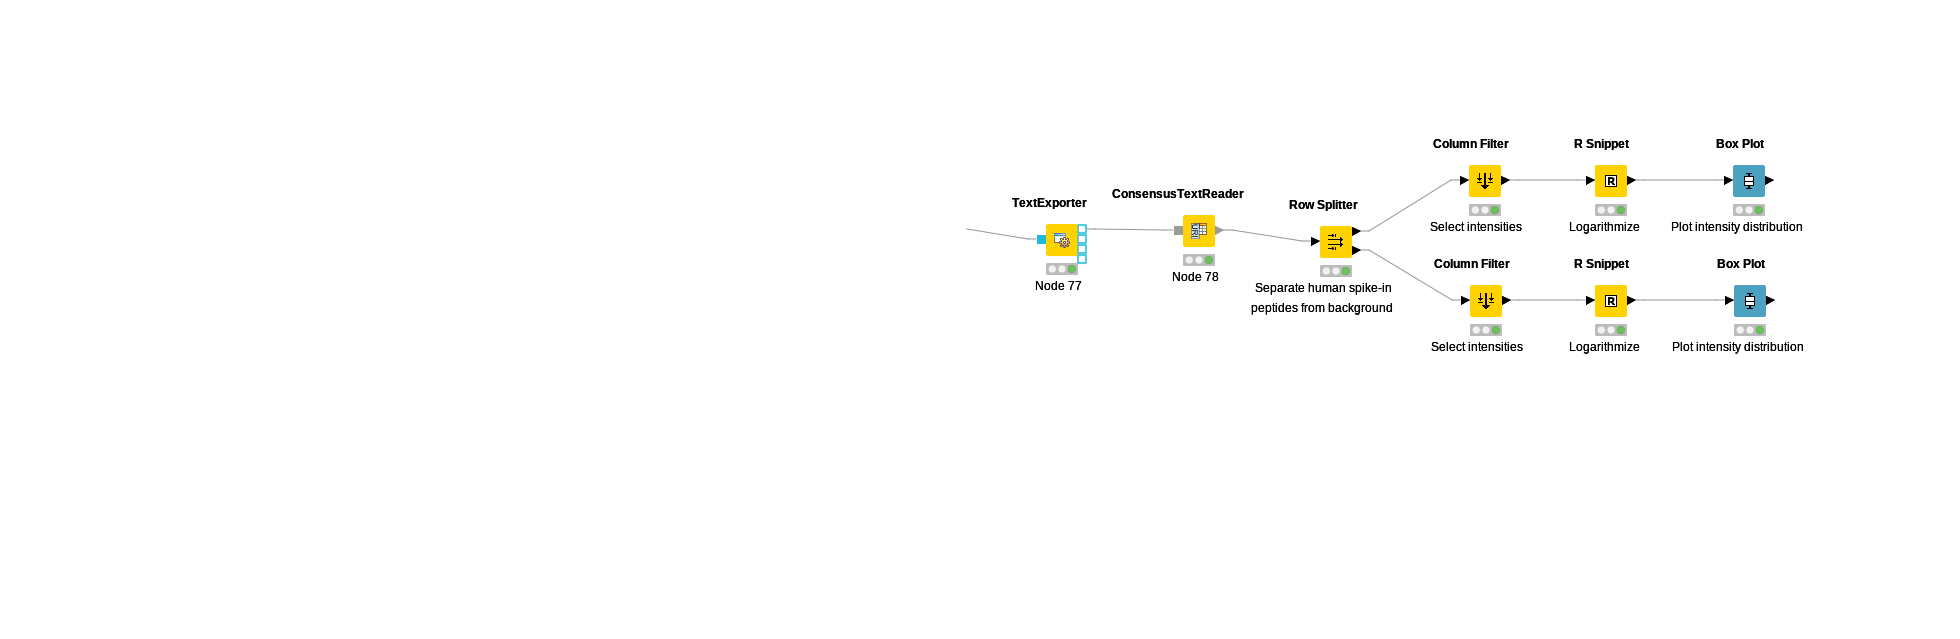
\includegraphics[width=0.85\textwidth]{graphics/labelfree/data_analysis.png}
  \caption{Simple KNIME data analysis example for LFQ.}
  \label{fig:lfq_data_analysis}
\end{figure}

\begin{itemize}
    \item Now, let's say we want to plot the log intensity distributions of the human spike-in peptides for all input files. In addition, we will plot the intensity distributions of the background peptides.
    \item As shown in Fig. \ref{fig:lfq_data_analysis}, add a \KNIMENODE{Row Splitter} node (\menu{Data Manipulation > Row > Filter}) after \KNIMENODE{ConsensusTextReader}. Double-click it to configure. The human spike-in peptides have accessions starting with ``hum''. Thus, set the column to apply the test to: \textit{accessions}, select pattern matching as matching criterion, enter \textit{hum*} into the corresponding text field, and check the \textit{contains wild cards} box. Press OK and execute the node.
    \item \KNIMENODE{Row Splitter} produces two output tables: the first one contains all rows from the input table matching the filter criterion, and the second table contains all other rows. You can inspect the tables by right-clicking and selecting \textit{Filtered} and \textit{Filtered Out}. The former table should now only contain peptides with a human accession, whereas the latter should contain all remaining peptides (including unidentified ones).
    \item Now, since we only want to plot intensities, we can add a \KNIMENODE{Column Filter} node \\ \menu{Data Manipulation > Column > Filter}, connect its input port to the \textit{Filtered} output port of the \KNIMENODE{Row Filter}, and open its configuration dialog. We could either manually select the columns we want to keep, or, more elegantly, select \textit{Wildcard/Regex Selection} and enter \textit{intensity\_?} as the pattern. KNIME will interactively show you which columns your pattern applies to while you're typing.
    \item Since we want to plot log intensities, we will now compute the log of all intensity values in our table. The easiest way to do this in KNIME is a small piece of R code. Add an \KNIMENODE{R Snippet} node \menu{R} after \KNIMENODE{Column Filter} and double-click to configure. In the \textit{R Script} text editor, enter the following code:
        \begin{lstlisting}
            x <- knime.in       # store copy of input table in x
            x[x == 0] <- NA     # replace all zeros by NA (= missing value)
            x <- log10(x)       # compute log of all values
            knime.out <- x      # write result to output table
        \end{lstlisting}
    \item Now we are ready to plot! Add a \KNIMENODE{Box Plot} node \menu{Views} after the \KNIMENODE{R Snippet} node, execute it, and open its view. If everything went well, you should see a significant fold change of your human peptide intensities across the three runs.
    \item In order to verify that the concentration of background peptides is constant in all three runs, you can just copy and paste the three nodes after \KNIMENODE{Row Splitter} and connect the duplicated \KNIMENODE{Column Filter} to the second output port (\textit{Filtered Out}) of \KNIMENODE{Row Splitter}, as shown in Fig. \ref{fig:lfq_data_analysis}. Execute and open the view of your second \KNIMENODE{Box Plot}.
    \item That's it! You have constructed an entire identification and label-free quantification workflow including a simple data analysis using KNIME!
\end{itemize}
 
%The output of the node should now be compatible with most of the nodes of the KNIME base as well as the R nodes, which leaves room for you to play with these.
%Possible analyses include:

%\begin{task}
%Filtering (\KNIMENODE{Row Filter}, \KNIMENODE{Rule-based Row Filter}) or grouping (\KNIMENODE{GroupBy}; e.g. by charge) of the identified peptides/proteins.
%\end{task}
%\begin{task}
%Statistical analysis with \KNIMENODE{R Snippet} nodes or the nodes from the KNIME Statistics package.
%\end{task}
%\begin{task}
%Plotting of the (cumulative) distribution of q-values, quality scores (of the consensus features) or other peptide hit properties using \KNIMENODE{R View} nodes or the standard KNIME nodes for plotting (which include interactive functionality).
%\end{task}

\subsection{Identification \& Quantification of the iPRG2015 data with subsequent MSstats analysis}
Advanced downstream data analysis of quantitative mass spectrometry-based proteomics data can be performed using MSstats ~\cite{Choi2014MSstats}. This tool can be combined with an OpenMS preprocessing pipeline (e.g. in KNIME). The OpenMS experimental design is used to present the data in an MSstats-conformant way for the analysis. In this tutorial, we would like to present an example how to utilize these resources when working with quantitative label-free data. Therefore, we describe how to use OpenMS and MSstats in the analysis of the ABRF iPRG2015 dataset~\cite{Choi2017iPRG}.

\note{Due to runtime constrictions in the tutorial session only the conversion process and the downstream analysis will be presented in further detail.}

\subsubsection{Excursion MSstats}
The R package MSstats can be used for statistical relative quantification of proteins and peptides in mass spectrometry-based proteomics. Supported are label-free as well as labeled experiments in combination with data-dependent, targeted and data-independent acquisition. Inputs can be identified and quantified entities (peptides or proteins) and the output is a list of differentially abundant entities, or summaries of their relative abundance. It depends on accurate feature detection, identification and quantification which can be performed e.g. by an OpenMS workflow. 

\noindent In general MSstats can be used for data processing \& visualization, as well as statistical modeling \& inference. Please see ~\cite{Choi2014MSstats} and http://msstats.org/ for further information.

\subsubsection{Dataset}
The iPRG (Proteome Informatics Research Group) dataset from the study in 2015, as described in ~\cite{Choi2017iPRG}, aims at evaluating the effect of statistical analysis software on the accuracy of results on a label-free quantification experiment on proteins. The data is based on four artificial samples of known composition (background: 200\,ng \emph{S. cerevisiae}), which were spiked with different quantities of individual digested proteins, whose identifiers were masked for the competition as yeast proteins in the provided database (see table \ref{t:dataset_iPRG}).

\renewcommand{\arraystretch}{1.2} %% increase row height a little
\begin{table}[!ht]
\centering
\small
\caption{Samples (background: 200\,ng \emph{S. cerevisiae}) with spiked-in proteins in different quantities [fmols]}
\label{t:dataset_iPRG}
\begin{tabular}{llll|llll}
  &                          &                              &                                      & \multicolumn{4}{c}{Samples}            \\
\hline 
  & \multicolumn{1}{c}{Name} & \multicolumn{1}{c}{Origin}   & \multicolumn{1}{c}{Molecular Weight} & \multicolumn{1}{c}{1} & 2   & 3  & 4   \\
\hline
\hline
A & Ovalbumin                & \textit{Egg White}   & 45 KD                                 & 65                    & 55  & 15 & 2   \\
\hline
B & Myoglobin                & \textit{Equine Heart}        & 17 KD                                 & 55                    & 15  & 2  & 65  \\
\hline
C & Phosphorylase b          & \textit{Rabbit Muscle}       & 97 KD                                 & 15                    & 2   & 65 & 55  \\
\hline
D & Beta-Glactosidase        & \textit{Escherichia Coli}    & 116 KD                                & 2                     & 65  & 55 & 15  \\
\hline
\hline
E & Bovine Serum Albumin     & \textit{Bovine Serum}        & 66 KD                                 & 11                    & 0.6 & 10 & 500 \\
\hline
F & Carbonic Anhydrase       & \textit{Bovine Erythrocytes} & 29 KD                                 & 10                    & 500 & 11 & 0.6 \\
\hline
\end{tabular}
\end{table}

\subsubsection{Identification and Quantification}

\begin{figure}[htbp]
  \centering
  \includegraphics[width=1\textwidth]{graphics/labelfree/iPRG/iPRG_lfq.png}
  \caption{KNIME data analysis of iPRG LFQ data.}
  \label{fig:iPRG_lfq}
\end{figure}

\noindent The iPRG LFQ workflow (Fig. \ref{fig:iPRG_lfq}) consists of an identification and a quantification part. The identification is achieved by searching the computationally calculated MS2 spectra from a sequence database (\KNIMENODE{Input File} node, here with the given database from iPRG, \directory{\IPRGFOLDER / database / iPRG2015\_target\_decoy\_nocontaminants.fasta}) against the MS2 from the original data (\KNIMENODE{Input Files} node with all mzMLs following \directory{\IPRGFOLDER / datasets / JD\_06232014\_sample*.mzML}) using the \KNIMENODE{OMSSAAdapter}.
\note{If you reproduce at home, you have to download the iPRG data in mzML format and perform Peakpicking on it. Or convert and pick the raw data with msconvert.}
Afterwards the results are scored using the \KNIMENODE{FalseDiscoveryRate} and filtered to obtain only unique peptides (\KNIMENODE{IDFilter} TODO why? restriction of MSstats?). The quantification is achieved by the \KNIMENODE{FeatureFinderCentroided}, which performs feature finding on the maps. In the end the quantification results are combined with the filtered identification results (\KNIMENODE{IDMapper}). Further a linear retention time alignment is performed (\KNIMENODE{MapAlignerPoseClustering}), followed by the feature linking process (\KNIMENODE{FeatureLinkerUnlabledQT}). The \KNIMENODE{ConsensusMapNormalizer} is used to normalize the intensities via robust regression over a set of samples (maps) and the \KNIMENODE{IDConflictResolver} assures that only one identification (best score) is associated with a feature. The output of this workflow is a consensusXML file, which can now be converted using the \KNIMENODE{MSstatsConverter} (see \ref{sec:MSstatsConversion}). 

\subsubsection{Experimental design}
\noindent The downstream analysis can be performed using MSstats. In this case an experimental design has to be specified for the OpenMS workflow. The structure of the experimental design used in OpenMS in case of the iPRG dataset is specified in table \ref{t:Experimental_design_iPRG}. Further, an explanation of the variables can be found in table \ref{t:Experimental_design_exp}. 

\begin{table}[!ht]
\centering
\small
\caption{OpenMS Experimental design for the iPRG2015 dataset. Caution, in the original filenames, the first sample had a hyphen "-" as a separator between sample and biological replicate, the rest of the files had an underscore "\_". The common prefix was omitted.}
\label{t:Experimental_design_iPRG}
\begin{tabular}{lllll}
Fraction\_Group & Fraction           & Spectra\_Filepath     & Label & Sample \\
1               & 1                  & Sample1-A             & 1     & 1      \\
2               & 1                  & Sample1-B             & 1     & 2      \\
3               & 1                  & Sample1-C             & 1     & 3      \\
4               & 1                  & Sample2-A             & 1     & 4      \\
5               & 1                  & Sample2-B             & 1     & 5      \\
6               & 1                  & Sample2-C             & 1     & 6      \\
7               & 1                  & Sample3-A             & 1     & 7      \\
8               & 1                  & Sample3-B             & 1     & 8      \\
9               & 1                  & Sample3-C             & 1     & 9      \\
10              & 1                  & Sample4-A             & 1     & 10     \\
11              & 1                  & Sample4-B             & 1     & 11     \\
12              & 1                  & Sample4-C             & 1     & 12     \\
                &                    &                       &       &        \\
                &                    &                       &       &        \\
Sample          & MSstats\_Condition & MSstats\_BioReplicate &       &        \\
1               & 1                  & 1                     &       &        \\
2               & 1                  & 2                     &       &        \\
3               & 1                  & 3                     &       &        \\
4               & 2                  & 1                     &       &        \\
5               & 2                  & 2                     &       &        \\
6               & 2                  & 3                     &       &        \\
7               & 3                  & 1                     &       &        \\
8               & 3                  & 2                     &       &        \\
9               & 3                  & 3                     &       &        \\
10              & 4                  & 1                    &       &        \\
11              & 4                  & 2                   &       &        \\
12              & 4                  & 3                    &       &       
\end{tabular}
\end{table}

\begin{table}[!ht]
\centering
\small
\caption{Experimental design explanation}
\label{t:Experimental_design_exp}
\begin{tabularx}{\textwidth}{l|X}
\textbf{variables} & \textbf{value} \\ 
\hline \\
\textit{Fraction\_Group} &  Index used to group fractions and source files.  \\
\textit{Fraction} & 1st, 2nd, .., fraction. Note: All runs must have the same number of fractions. \\
\textit{Spectra\_Filepath} & Path to mzML files \\
\textit{Label} & label-free: always 1 \\
\textit{} & TMT6Plex: 1...6 \\
\textit{} & SILAC with light and heavy: 1..2 \\
\textit{Sample} & Index of sample measured in the specified label X, in fraction Y of fraction group Z. \\
\textit{Conditions} & Further specification of different conditions (e.g. MSstats\_Condition; MSstats\_BioReplicate) \\
\end{tabularx}
\end{table}

\noindent The conditions are highly dependent on the experiment and which kind of analysis you want to use. For the MSstats analysis it has to be clear which sample belongs to which condition and if there are biological replicates. This can be specified in further condition columns as shown in table \ref{t:Experimental_design_exp}.

\subsubsection{Conversion and downstream analysis}
\label{sec:MSstatsConversion}

Conversion and downstream analysis 
blabla workflow, 
The data can be found in "example data" , "iPRG" called iPRG\_lfq.consensusXML
\\
How to use the workflow. 
\\
Add Figure of complete iPRG workflow 
\\
The \KNIMENODE MSstatsConverter can be used to Converter the processed information into the format needed for MSstats analysis (see Fig y).  
\\
Description where the data is and how to use it. 
\\
\note{For further inspiration you might want to take a look at the more advanced KNIME data analysis examples in the metabolomics tutorial.}


\newpage{}

%%%%%%%%%%%%%%%%%%%%%%%%%%%%%%%%%%%%%%%%%%%%%%%%%%%%%%%%%%%%%%%%%%%%%%%%%%%
%\newpage

\bibliographystyle{phreporturl}
\bibliography{handout}

\end{document}
